\subsection{Генерация синтетических аннотированных данных}

В этом разделе описан процесс генерации синтетических аннотированных данных. Исходная последовательность $s_k = \{x_1, x_2, \ldots, x_{n_k}\}$ — это токенизированное $k$-е предложение с ошибками, целевая последовательность — токенизированное $k$-е предложение без ошибок $t_k = \{y_1, y_2, \ldots, y_{m_k}\}$, где $n_k$ и $m_k$ — длины исходной и целевой последовательностей соответственно.

В нашей формулировке задача сводится к поиску редакционного предписания.

Используется расстояние Левенштейна, которое определяется как минимальное число операций \textit{вставки} (append), \textit{удаления} (delete) и \textit{замены} (replace), необходимых для преобразования одной последовательности в другую.

\begin{figure}[h]
  \centering
  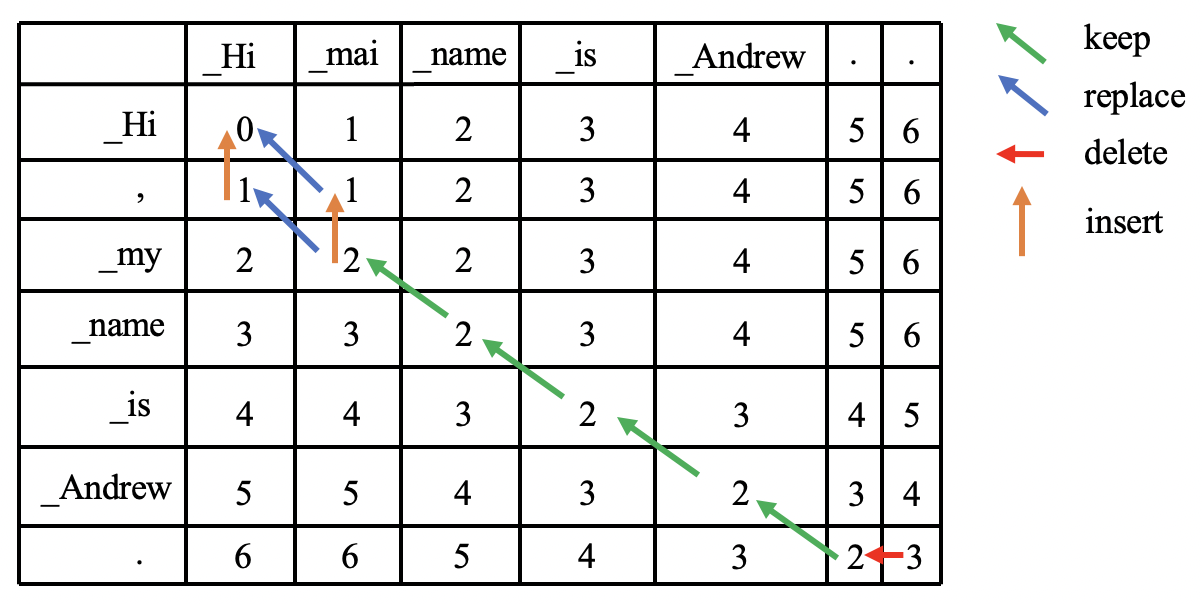
\includegraphics[width=\linewidth]{images/backtracking.png}
  \caption{Матрица Левенштейна и редакционные предписания между исходной и целевой последовательностями. Можно заметить, что существует несколько вариантов редакионных предписаний.}
  \label{fig:backtracking}
\end{figure}

Расстояние Левенштейна между исходной и целевой последовательностями эффективно вычисляется с помощью двумерной матрицы, которая заполняется с использованием алгоритма динамического программирования. Пусть $D_{i,j}$ — это расстояние редактирования между префиксами $s_k[0..i]$ и $t_k[0..j]$ длины $i$ и $j$, при этом $D_{0,j} = 0$ и $D_{i,0} = 0$. Остальные значения определяются следующим рекуррентным соотношением:

\[
D_{i,j} = 
\begin{cases} 
    D_{i-1, j-1}, & \text{если } s_k[i] = s_k[j] \\
    1 + \min \begin{cases} 
        D_{i-1, j}, \\
        D_{i, j-1}, \\
        D_{i-1, j-1} 
    \end{cases}, & \text{иначе}
\end{cases}
\]

На рисунке~\ref{fig:backtracking} показана матрица расстояний между префиксами токенизированного исходного предложения <<Hi mai name is Andrew..>> и токенизированного целевого предложения <<Hi, my name is Andrew.>>. Расстояние Левенштейна между исходной и целевой последовательностями отображается в правом нижнем углу матрицы и равно 3.

Редакционное предписание — это последовательность правил (\textit{keep}, \textit{replace}, \textit{append}, \textit{delete}) минимальной длины, описывающая действия, необходимые для получения целевой последовательности из исходной.

Чтобы найти эталонные корректирующие преобразования, необходимо определить редакционное предписание. Как показано на рисунке~\ref{fig:backtracking}, предписание можно получить с помощью обратного прохода по рассчитанной матрице расстояний. Начиная с правого нижнего угла таблицы, строим пути ко всем соседним ячейкам, соответствующим меньшим подзадачам и меньшим расстояниям редактирования. Движение вверх соответствует вставке подслова в исходную последовательность (\textit{append}), влево — удалению подслова (\textit{delete}), по диагонали — замене (\textit{replace}) или сохранению без изменений (\textit{keep}), если подслова совпадают.

\textbf{Утв. Количество редакционных предписаний соответствует количеству путей в графе подзадач с минимальной стоимостью.}

Например, для нашего случая существует два редакционных предписания:  
\{\textit{delete} \textbf{.}; \textit{append} \textbf{\_my}; \textit{replace} \textbf{\_mai} на \textbf{,}\}  
и  
\{\textit{delete} \textbf{.}; \textit{append} \textbf{,}; \textit{replace} \textbf{\_mai} на \textbf{\_my}\}.  
Таким образом, нам необходимо определить оптимальное редакционное предписание. Ввиду краткости правила \textit{keep} опущены.

Обозначим через $EP_k = \{e_{1}, e_{2}, \ldots, e_{o_k}\}$ множество редакционных предписаний для пары последовательностей $(s_k, t_k)$, где $o_k$ — количество предписаний для $k$-й пары.

Для определения оптимального редакционного предписания для $k$-й пары учитывается схожесть подслов при применении правила \textit{replace}. Пусть $R_l \in e_l, \, l \in \{1, 2, \ldots, o_k\}$ — множество всех правил \textit{replace} с мощностью $p_l$ для произвольного предписания $e_l$:
\begin{align*}
    R_l =\{replace\_{t_1}_{i}\_{t_2}_{i}\}_{i=0}^{p_l}, 
\end{align*}
где ${t_1}_i \in s_k$, ${t_2}_i \in t_k$.

Введём метрику схожести подслов:
\[
\sigma_l = \sum_{i=0}^{p_l} \text{LevenshteinDist}({t_1}_i, {t_2}_i),
\]
где $\text{LevenshteinDist}$ — функция, вычисляющая расстояние Левенштейна между ${t_1}_i$ и ${t_2}_i$ на уровне символов в подсловах.

Оптимальное предписание $e^*_l$ выбирается как:
\[
l = \arg\min \{\sigma_1, \sigma_2, \ldots, \sigma_{o_k}\}.
\]

Это и есть эталонная последовательность корректирующих преобразований для пары $(s_k, t_k)$.